Guidelines:
Seiten: 50
Präsentation: 30 min / Disskusion: 15 min
sonarqube als code scan

\section{Einleitung}

\subsection{Motivation}
\subsection{Unternehmen}
\subsection{Zielsetzung}
vielleicht im kapitel motivation?
\subsection{Aufbau der Arbeit}

- Outline your work such that readers who have not read subsequent chapters get an idea of what
  - your "problem domain" is (e.g. the software quality department of some company or the overarching research project you are working in)
  - the situation is (e.g. software tests at some company are done in complete manual fash-ion)
  - the complication / problem is (e.g. hotfixes have to be deployed totally untested in pro-duction)
  - what your approach is (e.g. establishing a concept and tool evaluation for continuously improving code coverage of automated tests)
  - what beyond the scope of your thesis is (e.g. also implementing a CICD pipeline)
  - what the actual core results are (e.g. how many tools have been evaluated)

From that it must clear, what your thesis'contribution actually is. Please delineate your contribution from every concept, method, tool, framework or whatever implementation your thesis took for granted and is built upon.

This chapter deliberately anticipates contents of the latter chapters but please refrain from spe-cific technical termsof your application domain or solution here. Trade technical accuracy for com-mon comprehensibility here. Write this chapter as a "management summary" and do not spend more than two to three pages here.

Also explain structure of your thesis, i.e., summarize the contents of each chapter in one sentence or paragraph and describe the overarching storyline, i.e., how chapters build upon each other.

\section{Anwendungsfeld Internet of Things}

ein grobes beispiel einet mqtt broker -> client anwendungs beschreiben
ein / mehrere broker (mehrere millionen clients zb MAN, darf ich das erzählen ?)
sehr viele iot clients
big downstream clients -> backends
industrial bereich

- Describe the (business) domain of your work. Ask yourself: What does the common reader need to know about the domain in order to understand the results of your work? For example, if you work contributes to the claim handling process of some insurance company, describe the common claim handling process.
- Please refrain from meandering explanations about details that have no relevance for later chapters (just in order to increase your page count).
- The header "Domain / Anwendungsfeld" is supposed to be replaced or extended with some more specific header like: "Domain 'Claim handling'"

\import{content/}{grundlagen}

\section{Problembeschreibung}

\subsection{Cluster Discovery}
discovery that works with hivemq cluster discovery (dns)
es kommen immer wieder neue nodes hinzu / weg zb bei rolling updates
load balancer muss diese nodes dynamisch hinzufüger oder entfernen
hivemq ist in der lage dynamische cluster joins zu machen also muss der lb auch in der lage dazu sein

\subsection{Langlebige TCP Verbindungen}
ein LB darf die tcp connections nicht terminieren bei einem update oder config änderung
mqtt setzt auf langlebiege tcp verbindungen! nicht wie bei http! bei http -> drain
-> ein drain bei mqtt kann tage dauern

load balancer with data plane api -> good docs
\subsection{Persistent Client Session}
mqtt clients haben viel session auf dem broker
bei einem reconnect wird ein client takeover ausgeführt -> teuer
clients möglichst immer zum selben broker routen
problem: iot clients haben oft sich ändernde ip adressen zb mobile geräte wie autos
\subsubsection{Client Takeover}
sehr teuer! die persistent client informationen müssen umgezogen werden auf neuen broker

\subsection{Ungleiche Lastverteilung}
mqtt clients sind unterschiedlich teuer (nicht wie bei http)
beispiel: wildcard subscription

\subsubsection{Downstream Clients}
\subsubsection{Lightweight Clients}
\subsubsection{Wildcard Subscriptions}

- Describe insufficiencies your project or thesis aims at. Example: "The automated parts of the claim handling process are susceptible to changes. Each change requires lots of man-ual steps in order to deploy these changes into production."
- Do not take the term "problem" too literal. Sometimes, your project or thesis just aims at im-proving a good status quo or pursues new waysand opportunities that arise due to new technological advances or trends. In this case, describe the status quo and where the op-portunities for improvement are.
- Exemplify things! Describe the problem / status quo by means of a specific scenario with concrete steps, concrete input and output data, etc., supported by expressive figures. Do not be afraid that the reader might think that your solution just works for that particular sce-nario. In general, readers can abstract from concrete details much easier that to envisionconcrete scenarios by interpreting overly generic, vague, meandering text passages. (More-over, writing in vague terms also leaves the impression that the writer either did not under-stand the problem for him- or herself or tries to blow up mundane issues.)

\section{Vobereiten und verwandte Arbeiten}
vielleicht brauche ich diese sektion gar nicht ?

\subsection{Load Balancer}
was für load balancer gibt es? was haben diese für eigenschaften?

\subsection{Shared Subscriptions}
diese lösen das problem der teuren clients ABER clients müssen dann möglichst optimal auf die broker verteilt werden
-> load balancer

iot mqtt threat model ? maybe show this ?

- If your work is based on preliminary work, then outline this preliminary work: "The de-ployment into production is itself semi-automatic. In a continuous integration pipeline..."
- Do some research forrelated work, e.g., commercial products, research prototypes or con-ceptual research that have the same or similar objectives like your work. Compare and de-lineate your work with/from the related work.
- Keep an eye on the proper citation of the works you are describing
- Conclude this chapter with some insufficiencies or shortcomings of the preliminary or related work. This should motivate the necessity of your work.

\section{Lösungskonzept}
nur das konzept WIE ich das lösen will zb. man kann wie clientid parsen mit einem WASM modul
in der nächsten section zeige ich dann den eigentlichen code welcher dies tut

\subsection{Envoy}
\subsubsection{Data-Plane API}
\subsubsection{Hot Restart}

\subsection{DNS Service Discovery}

\subsection{Weighted Round Robin}
\subsubsection{Overload Protection}
\subsubsection{Client Credits}
\subsubsection{Global Tasks}

\subsection{Sticky Session with Client ID}
\subsubsection{MQTT CONNECT}
\subsubsection{Envoy WASM Network Filter}

- This is supposed to be the core of your thesis or project. Describe your work from a con-ceptual viewpoint.
- Example: In case you have developed some prototypical tool in your bachelor thesis, demonstrate how it is employed in its business context. More concrete example: Assume that your contribution is a Maven-Build-Plugin that further automates the deployment of changes to the claim handling process into production. In this case show how the plugin is integrated in the overall (continuous) integration and deployment process, which human ac-tors are involved, which external systems and so on. Elaborate on subtle edge cases you had to deal with, e.g., possible outages of external systems.
- Usedi  agramswhere appropriate. Standard notations are better than informal box-and-line-diagrams. Typical standard notations for a solution concept are
  - Business Process Modelling Notation (BPMN) or UML activity diagrams, that depict a workflow in which your tool is used
  - UML component diagrams, where your tool is represented by just a single component (without its ingredients) together with connected external systems

\section{Architektur und Implementation}

\subsection{Envoy}
\subsubsection{Golang Data-Plane}
\subsubsection{DNS Service Discovery}
\subsubsection{HiveMQ Metriken}
\subsubsection{Weighted Round Robin}
\subsubsection{ClientID Network Filter}

\subsection{Deployment}
\subsubsection{HiveMQ}
\subsubsection{Envoy}

- Describe the realization of your concepts, in case you have actually developed some-thing.
- Elaborate on the software architecture of your tool, in case you have developed one. Use nested UML packages, components, and interfaces in a component diagram.
- If applicable, show the deploymentof your tool in a production environment. Use UML's deployment diagram notation.
- It must be clear from the architecture, what your thesis contributes and what it takes for granted like existing systems, code bases, libraries and frameworks. For example, you can decorate the components in a UML component diagram that you have implemented and those that you just used.
- Do not delve into ordinary details by, e.g., intensively describing a "p lain old Java-object (POJO)" in all its dreary getter-setter-details. Instead pick some interesting details and de-scribe them, e.g.,
  - if   you made extensive use of a certain design pattern, describe a single concrete appli-cation of it using, e.g., UML class diagrams or
  - if your work involves a complicated conversation pattern or protocol, explained it using a UML sequence diagram, state chart, activity diagram and the like or
  - if you have developed a central and canny algorithm, you may even show its implemen-tation in, e.g., Java code.
- Show how the result of your work actually looks like. In case of a tool, provide some screenshots together with some explanatory text.
- Describe the quantity of your work, e.g., in terms of lines of code or classes etc. Please just count your own hand-crafted code but not previously existing, imported or generated code.
- Describe the quality of your work, e.g., if you have developed a large web application, run some performance tests, depicts results and draw conclusions from them.

\section{Erprobung}

\subsection{Lastverteilung}

If possible, do an (external) evaluation of your work. If you have developed some kind of tool, let us-ers test it, gather their feedback and describe that here. (Negative feedback will not contribute to a downgrading).

\section{Zeitplanung und Arbeitspakete}

- In the initiation phase, we agree on work packages. Give a (tabular overview) of which work packages have been finalized
  - to what degree
  - and in which time frame
- Please described the unforeseen difficulties that resulted in unfinished or abandoned work packages


\section{Ausblick}

- Again, summarize your work. This time you can assume that reader have read the rest of the document, i.e., you are free to use even domain-specific terms.
- In case of a master thesis in "Technische Informatik", you will have to provide an addi-tional "technical report" in English of 4-8 pages (cf. examination regulation document, §28, 1d). It is okay for me if you use this technical report as the summary here.
- Usually, during your project or thesis new and extended questions arise that are not dealt with in your project or thesis due effort reasons. Please delineate these in the outlook.

BEISPIELE:

Figure \ref{fig:mender-integration} shows all microservices and their network connections.
\begin{figure}
    \centering
    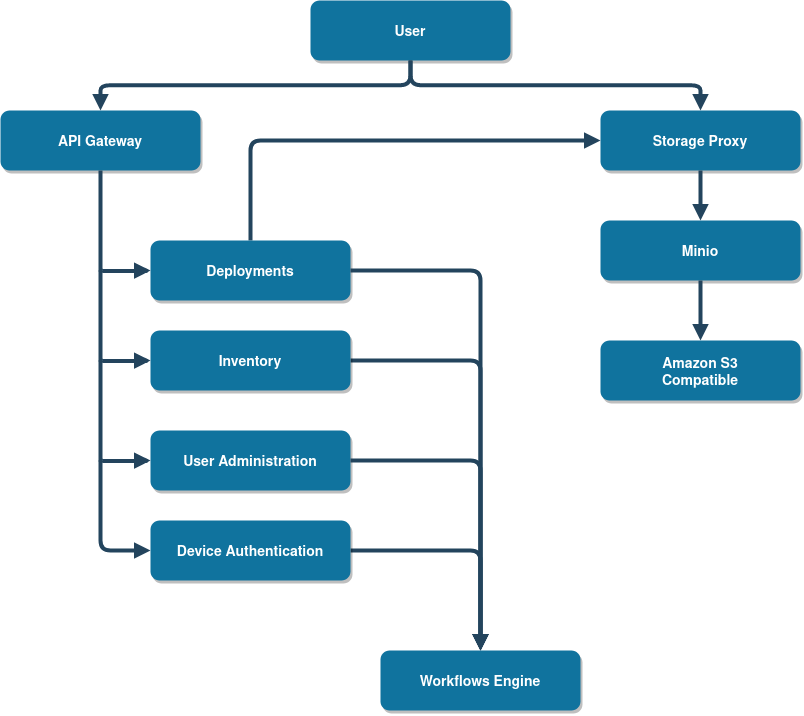
\includegraphics[scale=0.5]{images/integration-app.png}
    \caption{Mender Integration Server Architecture}
    \label{fig:mender-integration}
\end{figure}
Minio is a third-party object storage. It can either be used to serve uploaded content on its own or to proxy requests to Amazon S3 compatible cloud providers. All other services are mender application logic web services.
\newpage

\begin{figure}
    \import{gen/}{example}
    \caption{Example Code Listing}
    \label{code:example-label}
\end{figure}

Listing \ref{code:example-label} is a very good YAML file.
